\documentclass[a4paper,12pt]{article}

\usepackage{amsmath,amssymb,amsthm,bm}
\usepackage{subfigure}
\usepackage{graphicx}
\usepackage{url,booktabs}
\usepackage{multirow}
\usepackage{algpseudocode}
\usepackage{algorithm}
\usepackage{hyperref,xcolor}
\usepackage{indentfirst}
\setlength{\parindent}{1.25cm}

\usepackage[portuguese]{babel}      % para texto em Português
\usepackage[utf8]{inputenc}   % para acentuação em Português OU


\begin{document}

\title{
{\sf Primeira Avaliação de Análise Multivariada 2}:\\
}

\author{
Aluno: Adyla Conceição Alves Borges\\
Departamento de Estat\'istica,\\
Universidade Federal de Pernambuco, Brazil
}

%\affil{Departamento de Estat\'{\i}stica, Universidade Federal de Pernambuco, Brasil}

\maketitle



\section{Introdução}
\label{sec:INTRO} 

Este trabalho irá trabalhar com dados de imagem de satélite da região entre Concord e Stockton, na Califórnia, EUA. 

\begin{center}
\begin{figure}[H]
    \centering
    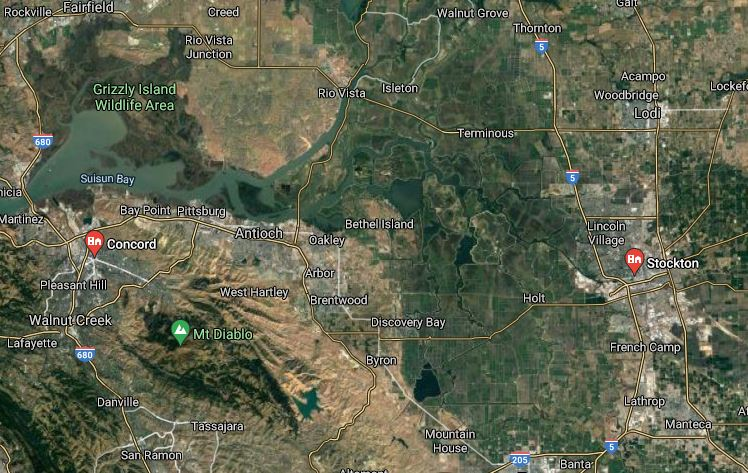
\includegraphics[width = 1 \textwidth]{satelite.JPG}
    \caption{Imagem de satélite da região entre Concord e Stockton, na Califórnia, EUA }
\end{figure}    
\end{center}

\section{Objetivo}

Tendo em vista todas as técnicas obtidas sobre dados multivariados e dados de imagem, iremos aplicá-la no referido banco de dados, afim de analisá-lo, utilizando principalmente análise de componentes principais e análise fatorial.

\section{Banco de dados}

Os dados utilizados neste trabalho são um conjunto de dados multiespectrais coletados do espaço. As bandas multiespectrais podem ser vistas abaixo, assim como suas resoluções espacias.


\begin{table}[ht]
\centering
\caption{Tipos de Bandas} \label{tab:exemplo}
\begin{tabular}{c c}
\hline
 \textbf{Banda} & \textbf{Tipo da banda}\\
\hline 
Band 2 & Blue \\
Band 3 & Green \\
Band 4 & Red \\
Band 5 & Near Infrared (NIR) \\
\hline
\end{tabular}
\end{table}

\begin{center}
\begin{figure}[H]
    \centering
    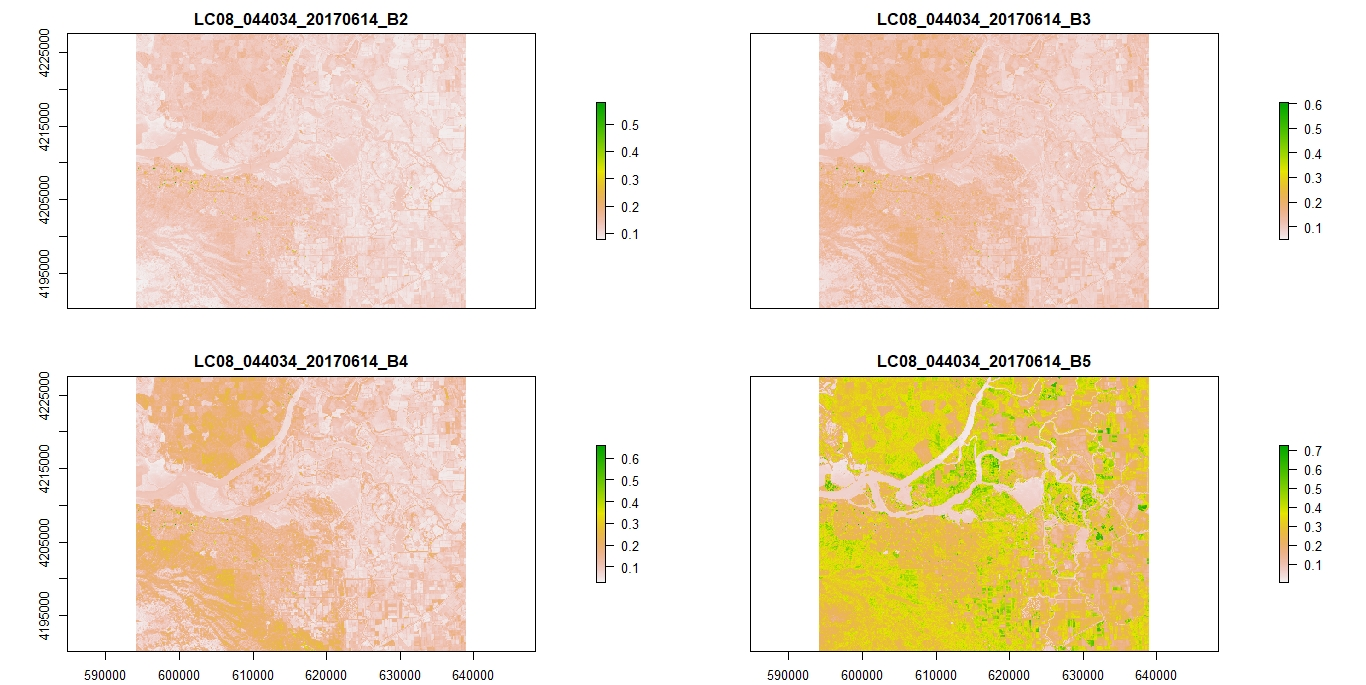
\includegraphics[width = 1 \textwidth]{banda colorida.jpeg}
    \caption{Representação das bandas coloridas}
\end{figure}    
\end{center}

\begin{center}
\begin{figure}[H]
    \centering
    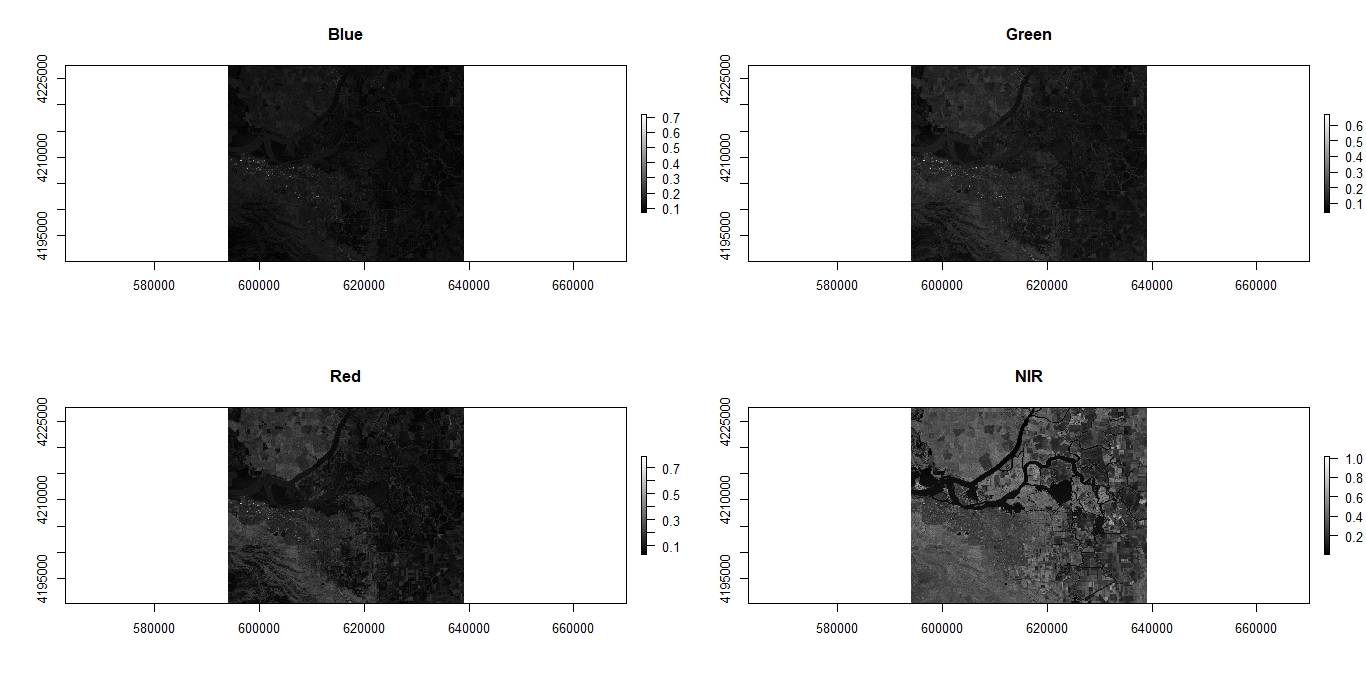
\includegraphics[width = 1 \textwidth]{banda pretobranco.jpeg}
    \caption{Representação das bandas em escala de cinza}
\end{figure}    
\end{center}


Ao verificar cada banda, é possivel combinar vários tipos de banda e assim obter uma nova imagem com um realçe específico para determinada área da banda.\newline
Logo em baixo podemos vê dois exemplos, onde algumas bandas foram combinadas. No primeiro exemplo, a banda 4 (Red), a banda 3 (Green) e a banda 2 (Blue), foram combinadas.\newline
A imagem obtida é semelhante a uma fotografia normal, chamada de cor verdadeira, ou seja, algo que se pareça com uma fotografia normal (vegetação em verde, água azul etc) Podemos observar isso na imagem abaixo

\begin{center}
\begin{figure}[H]
    \centering
    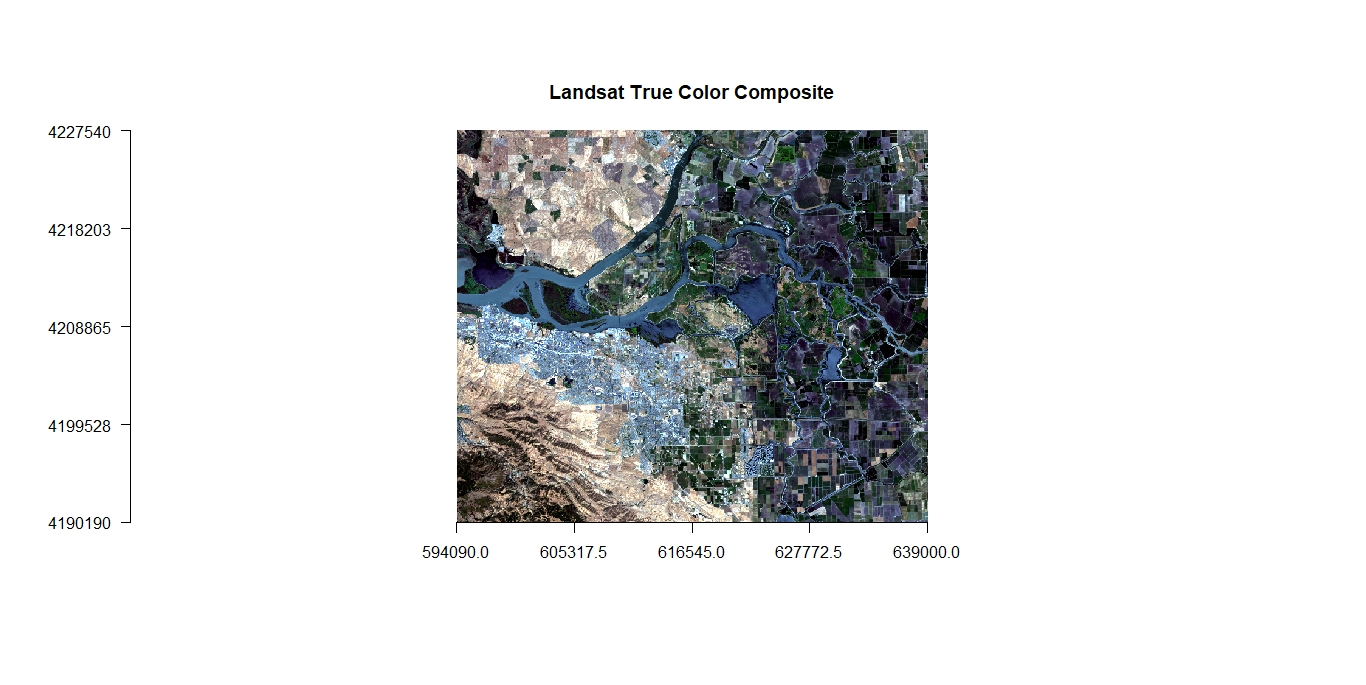
\includegraphics[width = 1 \textwidth]{comp 432.jpeg}
    \caption{Composição das bandas 4,3 e 2}
\end{figure}    
\end{center}

Ao combinarmos as bandas 5(NIR), 4 (Red) e 3 (Green), podemos observar uma imagem com uma cor chamada de falsa devido a sua coloração. Essa representação é utilizadas para visualizar vegetação, que é representada pela coloração vermelha.

\begin{center}
\begin{figure}[H]
    \centering
    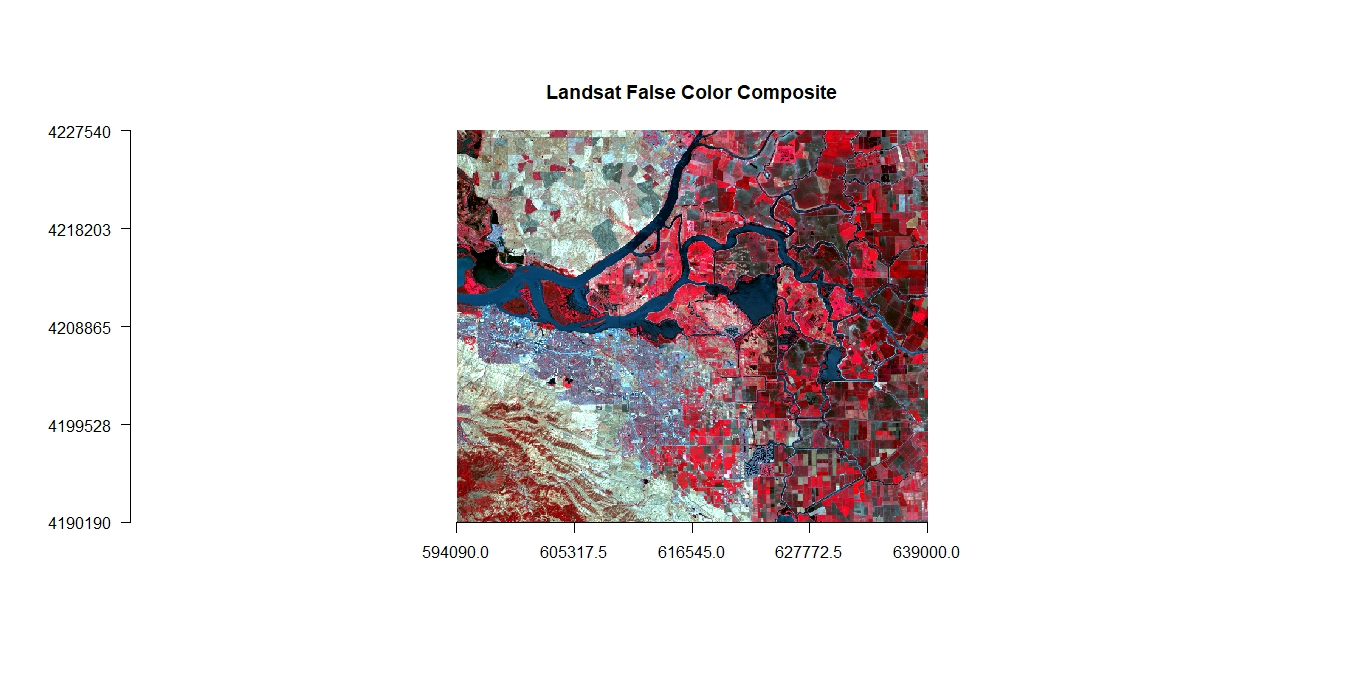
\includegraphics[width = 1 \textwidth]{comp 543.jpeg}
    \caption{Composição das bandas 5,4 e 3 }
\end{figure}    
\end{center}

Podemos ainda verificar a correlação entre as bandas. Pela matriz de correlação (tabela 2), podemos notar que existe uma alta correlação entre as bandas 2,3 e 4. Porém a banda 5 é a que representa uma menor correlação entre as outras bandas.

\begin{table}[ht]
\centering
\caption{Matriz de correlação} \label{tab:exemplo}
\begin{tabular}{c c c c c}
\hline
  & \textbf{Band 2} &  \textbf{Band 3} &  \textbf{Band 4} &  \textbf{Band 5}\\
\hline 
\textbf{Band 2} & 1 & 0.943 & 0.860 & 0.103 \\
\textbf{Band 3} & 0.943 & 1 & 0.952 & 0.355 \\
\textbf{Band 4} & 0.860 & 0.952 & 1 & 0.360 \\
\textbf{Band 5} & 0.103 & 0.355 & 0.360 & 1 \\
\hline
\end{tabular}
\end{table}

Pelo histograma podemos perceber também essa diferença. Quando observamos o comportamento dos dados, vemos que a distribuição dos dados das bandas 2,3 e 4 possuem uma assimetria a esquerda. Já a banda 5, possue uma maior variabilidade dos dados, ainda assim possue uma leve assimetria a esquerda.

\begin{center}
\begin{figure}[H]
    \centering
    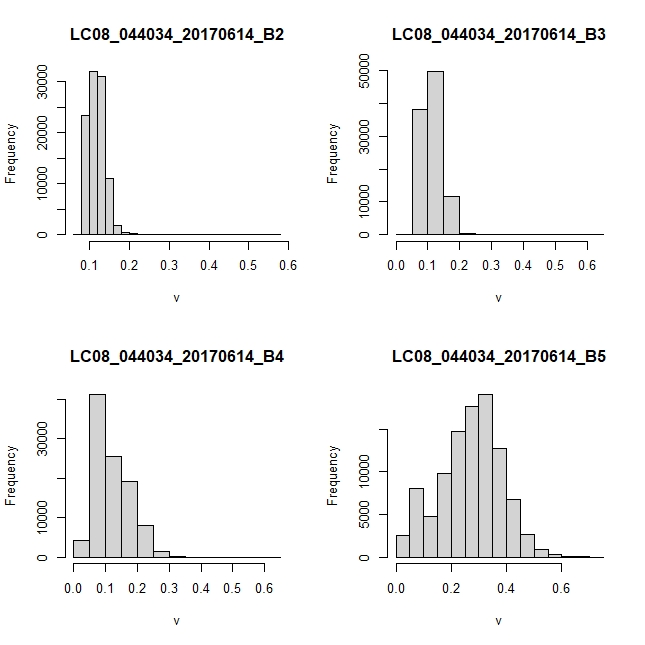
\includegraphics[width = 1 \textwidth]{hist.jpeg}
    \caption{Histograma das bandas 2, 3, 4 e 5}
\end{figure}    
\end{center}

\section{Análise de componentes principais}

Análise de componentes principais é uma técnica de análise multivariada que pode ser usada para analisar inter-relações entre  um grande número de variáveis e explicar essas variáveis em termos de suas componentes. Através de uma combinação linear padronizada das variáveis originais  e de uma decomposição espectral, onde a dimensionalidade dos dados é reduzida de tal forma que a perda de informações seja a mínima possível com a maior variância possível. Quando assumimos que o posto da matriz não singular é completo, utilizamos uma decomposição mais geral chamada de decomposição em valores singulares. Diferente da decomposição espectral que é feita sobre a matriz de variância e covariância dos dados, a decomposição em valores singulares é feita diretamente nos dados.\\

Através dos autovalores da matriz é possivel encontrar um resumo da contribuição de cada componente na descrição da variabilidade total. Essas contribuições podem ser vistas através do gráfico abaixo.\\

\begin{center}
\begin{figure}[H]
    \centering
    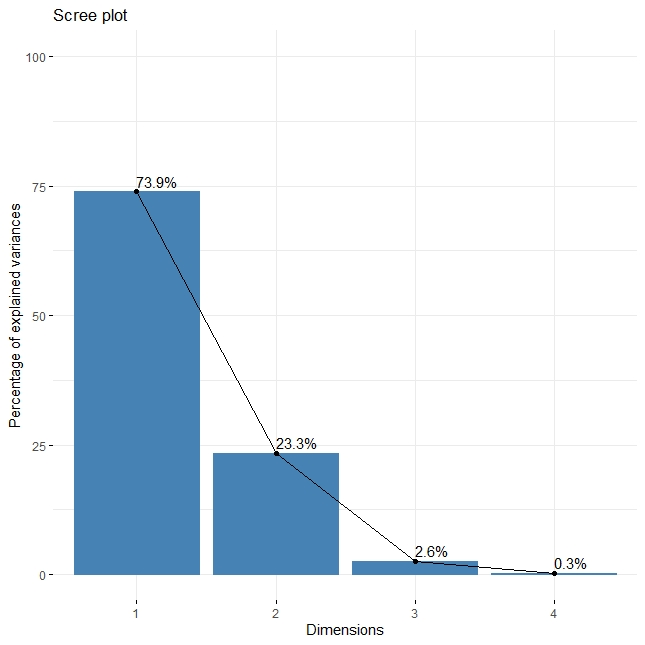
\includegraphics[width = 0.9 \textwidth]{boxplot.jpeg}
    \caption{Análise de autovalores}
\end{figure}    
\end{center}

Através do gráfico, podemos ver que as 4 bandas podem ser representadas apenas pelas 2 primeiras componentes principais, ou seja, podemos fazer uma redução de dimensionalidade de 4 para 2, visto que as duas primeira componentes principais conseguem explicar, pouco mais de 97$\%$ da variabilidade dos dados.\\

Para análisar a relação das bandas com as duas novas componentes principais, foi criado o círculo de correlações, que nada mais é do que um gráfico que representa as correlações entre variáveis e componentes.


\begin{center}
\begin{figure}[H]
    \centering
    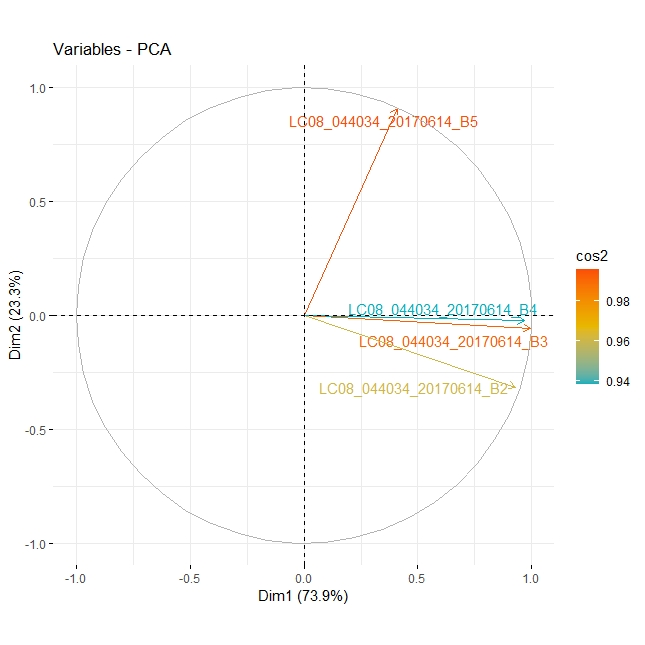
\includegraphics[width = 0.9 \textwidth]{PCA.jpeg}
    \caption{Variáveis PCA}
\end{figure}    
\end{center}

\begin{table}[ht]
\centering
\caption{Coordenada das variáveis} \label{tab:exemplo}
\begin{tabular}{c c c}
\hline
 \textbf{Banda} & \textbf{Dim. 1} & \textbf{Dim. 2}\\
\hline 
Band 2 & 0.9279410 & -0.31607369 \\
Band 3 & 0.9943053 & -0.05717209 \\
Band 4 & 0.9683449 & -0.02246141 \\
Band 5 & 0.4084262 & 0.91055522 \\
\hline
\end{tabular}
\end{table}


As componentes principais Dim 1 e Dim 2, seram as novas variáveis que iram representar as 4 bandas anteriores. Atavés da projeção de vetores, teremos um idéia de quais das 4 bandas estão sendo melhor representadas pelas novas componentes principais.\\

Com relação a Dim 1 (eixo x), podemos notar que todas as bandas estão sendo bem representadsa esse eixo, já essa componente consegue explicar 73,9 $\%$ da variabilidade dos dados.\\

Podemos notar ainda que todas as bandas estão correlacionadas positivamente com a componente Dim1. Sendo as bandas 2,3 e 4, as que são melhores representadas através da Dim1. Já que a Band 2 é representada com cerda de 92$\%$ pela PCA Dim1, a Band 4 com cerca de 96$\%$ e a Band 3 sendo a melhor representada pela PCA Dim1, com pouco mais de 99$\%$, sendo quase totalmente representada por ela.\\

Observando agora o eixo y (Dim2), podemos observar que a banda 5 é a melhor representada pela váriavel Dim2, possuindo uma correlação positiva entre ela e sendo representada com cerca de 91$\%$ pela PCA Dim2. Já as outras bandas possuem um correlação negativa com a várivel Dim2.\\

As correlações também podem ser verificadas no gráfico de variáveis PCA, já que as que estão no 4º quadrante são influênciadas de forma negativa pela Dim 2 e a Band 5 que está no 1º quadrante é influênciada de forma positiva.


\section{Método Biplot}

Biplot é uma técnica multivariada proposta por Gabriel (1971), com o objetivo de
representar graficamente uma matriz de dados, de tal forma que esta representação permita visualizar em um plano as relações e inter-relações entre as linhas e colunas desta matriz.  Após reduzir a dimensionalidade, podemos ver com o biplot a relação que os indivíduos tem entre si e a relação que as variáveis tem entre si, ou seja, essa fatoração ajuda a entender os dados tanto pelas suas variáveis como para seus indivíduos.\\

O biplot para todos os dados 1.863.765 ficou da seguinte forma:

\begin{center}
\begin{figure}[H]
    \centering
    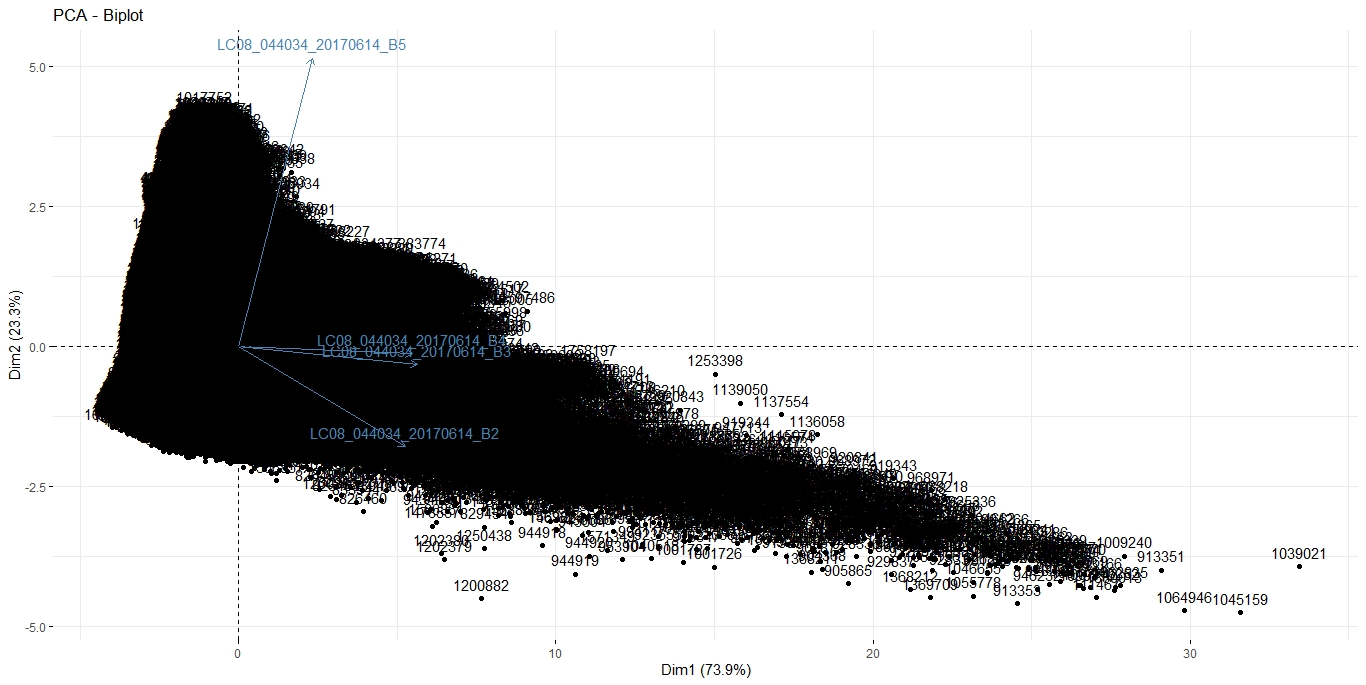
\includegraphics[width = 0.9 \textwidth]{total.jpeg}
    \caption{Gráfico Biplot}
\end{figure}    
\end{center}

Como podemos observar, por conter muitos dados fica um pouco dificil interpretar o gráfico. Por isso optou-se por retirar amostras das matriz para podermos visualizar melhor o comportamento dos dados. As amostras retiradas foram de tamanho 100, 150, 200 e 500 e podem ser vistas respectivamente abaixo.

\begin{center}
\begin{figure}[H]
    \centering
    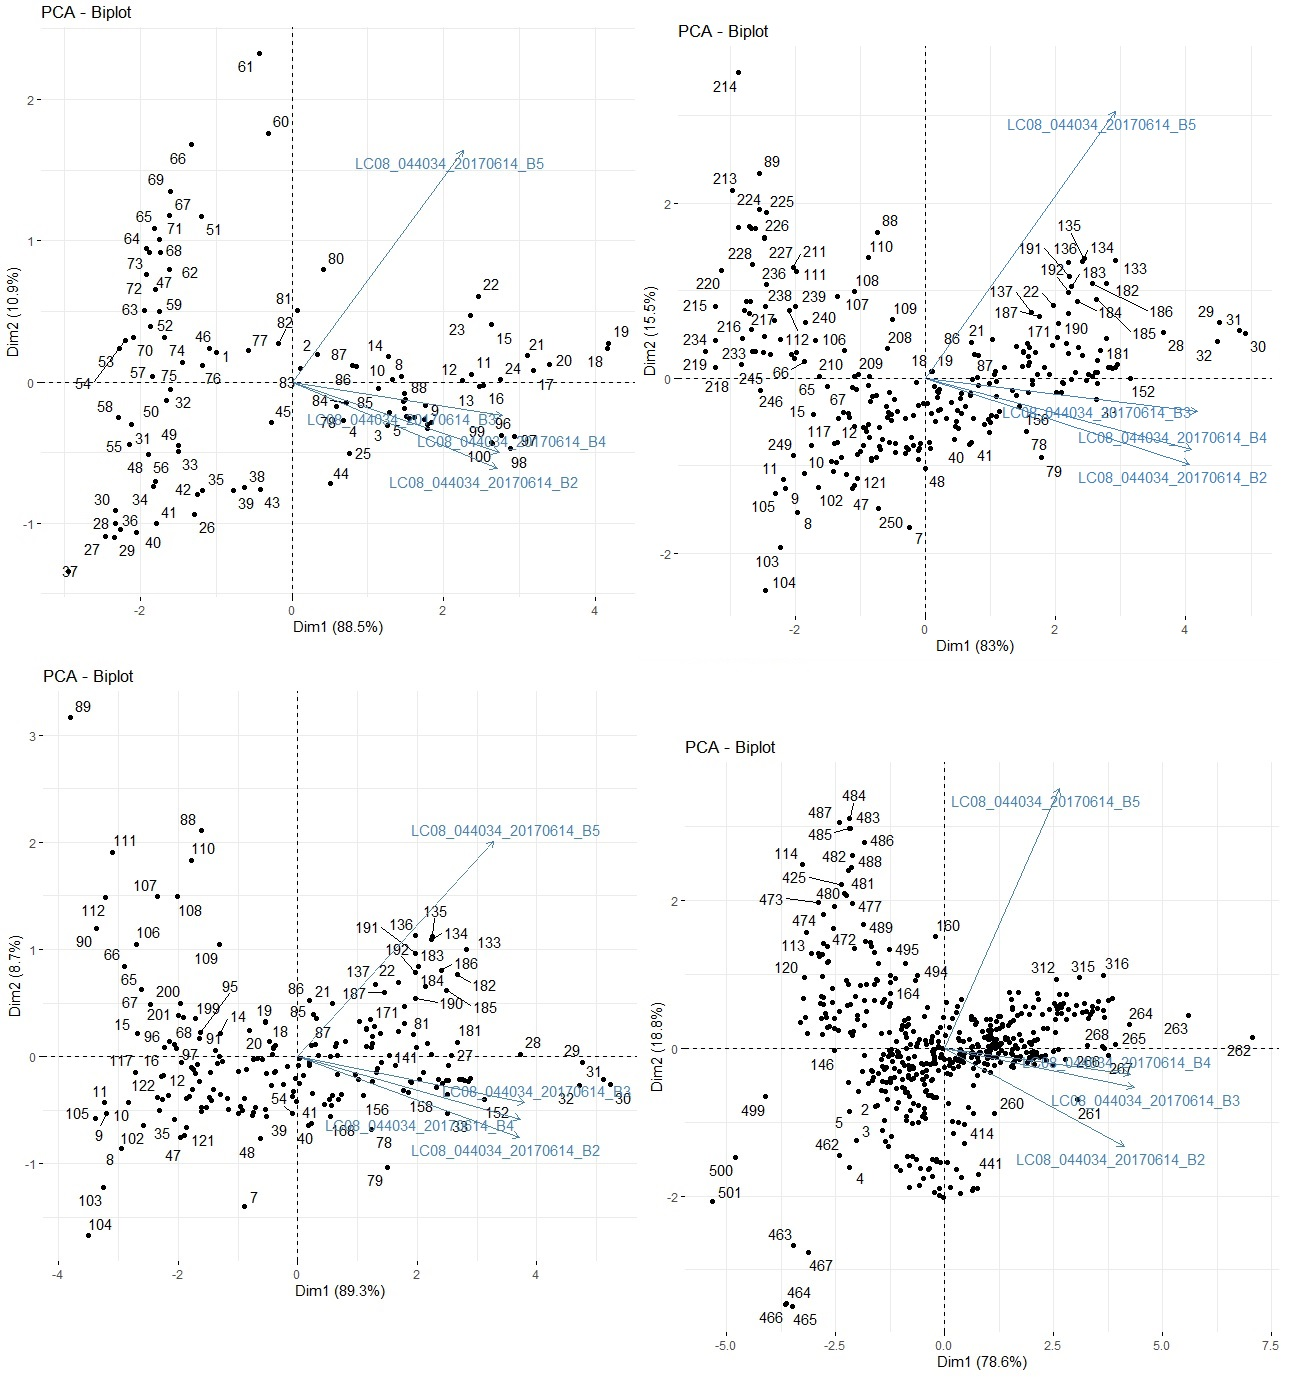
\includegraphics[width = 0.9 \textwidth]{Sem título.jpg}
    \caption{Biplot das amostras 100,150,200 e 500}
\end{figure}    
\end{center}

Por meio dos biplot apresentados, é possível ver de uma forma geral que a  maior variabilidade se concentram nas bandas 2,3 e 4. Pois a maioria dos pontos estão mais concentrados perto dessas bandas, o que não acontece com a banda 5. Logo, nota-se que a banda 5 tem um comportamento diferente das demais, uma vez que ela está sempre mais distante da concentração dos pontos.


\section{Análise Fatorial}

A análise fatorial é considerada uma extensão da análise de componentes principais e tem como principal objetivo descrever, atráves de fatores, uma matriz de covariância de um vetor aleatório. A matriz de covariância vai ser uma partição de dias matrizes, uma com valores latentes(gama) e a outra com a variabilidade do erro. Os erros são não correlacionados e a quantidade de fatores é menor do que a quantidade observada originalmente.\\

Para este trabalho, foi aplicado uma análise fatorial e testada a adequacidade de um modelo fatorial para verificar se uma determinada quantidade de fatores é suficiente para descrever todas as bandas nas quais estamos trabalhando. Como estamos trabalhando com 4 bandas, foram realizados testes para apenas 1 fator. Na tabela a seguir podem ser vistos a relação entre bandas e fator.\\


\begin{table}[ht]
\centering
\caption{Fatores} \label{tab:exemplo}
\begin{tabular}{c c c}
\hline
 \textbf{Banda} & \textbf{Fator 1} \\
\hline 
Band 2 & 0.943 \\
Band 3 & 0.998 \\
Band 4 & 0.953 \\
Band 5 & 0.348 \\
\hline
\end{tabular}
\end{table}

Através da tabela 3 podemos observar que as bandas 2,3 e 4 sãobem relacionados com o fator 1, já que possuem uma relação maior que 90$\%$. Porém a banda 5 tem uma baixa relação com o fator 1 sendo de aproximadamente 35$\%$. Após a realização do teste de hipótese, para verificar se as relações são significativas ou não, vemos que as mesma não foram significativas, já que rejeitamos o teste de hipótese (p-valor = 0) de que o apenas um fator é suficiente para representar as quatro bandas.

\begin{center}
\begin{figure}[H]
    \centering
    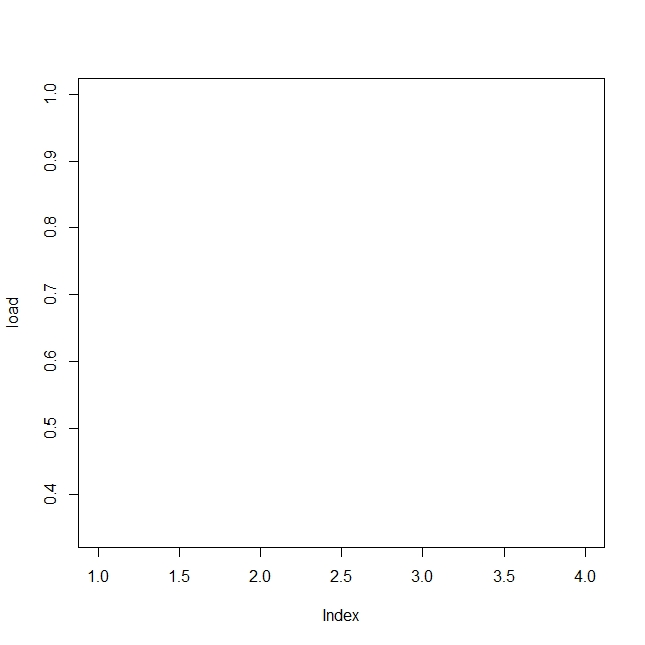
\includegraphics[width = 0.9 \textwidth]{1fator.jpeg}
    \caption{Gráfico de fatores}
\end{figure}    
\end{center}






























































\end{document}